This sections describes the simulation interaction between agents. Of the
research directions presented in this chapter, it is definitely the most
maleable. Deciding how a simulation is structured from an interactions
standpoint is a delicate balance of known necessity and perceived future
needs. There are basic decisions to make: do you want a system with discrete
material transfers or continous material flows? Discrete transfers more closely
match reality and may provide insights in that regard, however the require more
of their modeling apparatus due to messaging needs and other structures. More
complex decisions include how one wants to determine connections between
facilities. Do we assign supplier-consumer pairs to facilities? Do we allow them
to change? Should the facility make such a decision? Should that decision be
affected by any other entities? Guerin's comment in \S\ref{sec:intro-benchmarks}
stems from this ``freedom''. These simulation-engine decisions comprise the
art-related portion of fuel cycle simulation. The goal is to make these
decisions in as informed a way as possible from our domain-level knowledge with
respect to our known and perceieved requirements. In general, we try to minimize
the sheer number of choices we make in this regard, instead relying on well
known and well documented practices of computer scientists and systems
engineers.

\Cyclus has an additional goal in that we wish our core simulation
infrastructure to be as flexible as possible. Given a few basic tennets of agent
interaction, other developers should be able to create a new agent to ``plug
in'' to the simulation. Accordingly, we must define a minimal set of behaviors
to sufficiently inform the simulation infructure to run the simulation. This
freedom allows us to run the simulation program and attach agents at run time,
effectively separating the simulation engine's functionality from the agents in
the simulation. From an ecosystem point of view, being an open source code and
having such capability allows expansion of the user and developer base into
areas and institutions concerned with security and privacy. Furthermore,
developers could participate both privately and publicly, e.g. adding general
capability to the \Cyclus core that is needed for some functionality without
specifying the internals. Such a community paradigm is shown in Figure
\ref{fig:community}.

\begin{figure}[htbp!]
  \begin{center}
    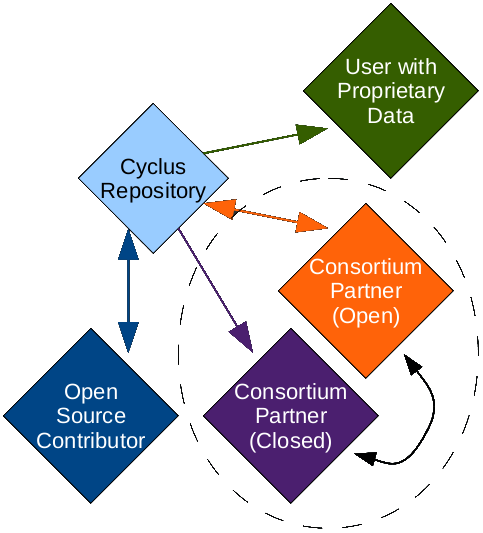
\includegraphics[height=8cm]{./chapters/research/community.png}
  \end{center}
  \caption{The Cyclus Participation Paradigm} 
  \label{fig:community}
\end{figure}

This open-source ecosystem further provides incentive to develop the agent-based
simulation architecture. Other developers can concentrate their efforts on
individual agent interaction, effectively ecapsulating developer requirements
for learning and interacting with the various simulation systems. Having decided
upon agent-based interactions, one must determine a way to govern these
interactions. We want to minimize agent dependency due to our above discussion,
so using preference-based network flow formulations provide us with a viable
solution technique that provides a consistent interface. The remainder of this
section describes how that market resoluation interface is informed by the
agents. Basic agent simulation intereaction, such as entering and leaving the
simulation are also described.

\subsection{Supply/Demand Resolution Mechanism}

The resolution of supply and demand at any given time step is the result of the
mathmatical program techniques described in \S\ref{sec:gfctp}; however, there
are simulation-engine details that must be described in order to set up that
problem. The proposed resolution mechanism occurs in nominally three steps. The
agent interactions include consumers and producers of a set of commodities and
progresses is steps or ``phases''.

The first phase allows consumers of commodities to denote both the quantity of a
commodity they need to consume as well as the target isotopics, or quality. This
action is considered a ``posting'' of demand to the market exchange. Consumers
are allowed to ``overpost'', i.e., request more quantity than they can actually
consume as long as a corrseponding capacity constraint accompanies this
posting. Further, consumers are allowed to post demand for multiple commodities
that may serve to meet the same combine capacity. For example, consider an LWR
that can be filled with MOX or UOX. It can post a demand for both, but must
define a preference over the set of possible commodities it can consume. Another
example is that of an advanced fuel fabrication facility, i.e., one that
fabricates fuel partially from separated material that has already passed
through a reactor. Such a facility can choose to fill the remaining space in a
certain assembly with various types of fertile material, including depleted
uranium from enrichment or reprocessed uranium from separations. Accordingly, it
could demand both commodities as long as it provides a corresponding constraint
with respect to total consumption. At the end of the posting phase, the market
exchange will have a set of consumption portfolio for each consumer. Each
consumption portfolio may be constituted by multiple consumption requests, and
each may have a detailed isotopic quality defined; however, there must be a
cardinal preference over the requests in the portfolio and an overall capacity
for the portfolio. 

%% Finally, the portfoloios themselves must be labeled as either
%% a belonging to service provider or service consumer. This is an important
%% distinction in the fuel cycle because of the notion of recycling. Take, for
%% instance, a repository. Such a facility ``consumes'' waste products, however it
%% can be also thought of as providing a commodity, e.g. ``storage space''. The
%% important distinction here is that the entity ``providing'' the fuel does not
%% necessarily care which repository it goes to; however, the repository may have
%% some preference over which fuel it accepts (based on heatload or radiotoxicity,
%% for example). This distinction manifests itself in the setting of the preference
%% function (see \S\ref{sec:cost-function}), which, in this case, would be managed
%% by the repository. Additional details are described below.

The second phase allows suppliers to ``respond'' to the set of consumption
portfolios. Each portfolio is comprised of requests for some set of
commodities. Accordingly, for each request, suppliers of that commodity denote
production capacities and an isotopic profile of the commodity they can
provide. This isotopic profile is part of a heuristic mechanism to assign more
fine-grained preferences among suppliers and consumers. Suppliers are allowed to
offer the null set of isotopics as their profile, effectively providing no
information. A supplier may have its production be constrained by more than one
parameter. For example, a processing facility may have both a throughput
constraint (i.e., it can only process material at a certain rate) and an
inventory constraint (i.e., it can only hold some total material). The
formulation provided in \S\ref{sec:gfctp} allows for multiple of such
constraints as long as they are linear functions of the demanded commodity
quantity. The phase

The second step allows supplier entities to respond to the board of posted
demands. In general, this step is simple: suppliers know which commodities they
produce and at what maximum capacity they produce them. Accordingly, responses
can be posted to each consumer requesting a resource in their production
category. In the current formulation, capacity restrictions must be linear
functions of the demand, but may depend on specific qualities of the demand
(e.g. uranium enrichment and SWUs), because these are static at solution time
and can thus be evaluated and modeled as a constant. Furthermore, a producer can
provide more than one such capacity restriction. For example, an enriched
uranium provider could have capacities related to both SWU and natural uranium
reserves. This posting is termed a "response for requests for bids" and
effectively defines the possible arcs between consumers and producers. It should
be noted that consumers can request different commodities to meet the same
demand, i.e., this is a multi-commodity problem.

The third step is for consumers and their managers to assign a preference score
to each bid. In our system, managers are institutions and regions, where each is
allowed to affect the overal preference through modifiers. The facilities
themselves set the base preference score, which can be simply a funciton of the
commodity or, in a more advanced way, a funciton of both the commodity and
quality thereof. For example, a facility can say apriori that it prefers wood
over coal, but a region can inform the preference that no coal is allowed. It is
at this step that timeliness can be assessed, i.e., a facility can give a
preference of 0 to a response that will arrive too late. It is also at this
stage that consumers can group bid responses. For example, a facility could say
that it will accept only an order of wood or only an order of coal. Furthermore,
it can denote that it will only accept whole orders, i.e. all of its order must
come from a single supplier. This models the reality of the fuel cycle, but
transforms the problem from a linear program (LP) to a mixed integer/linear
program (MILP). Finally, a cost translation mapping is applied to the set of
preferences in order to assume the form of a minimum cost problem. Both
formulations are described in \S\ref{sec:gfctp}.

\subsection{Facilities}

\subsection{Institutions}

\subsection{Regions}
